%!TEX root = ../Thesis.tex
%!TEX program = xelatex
\documentclass[../Thesis]{subfiles}

% 本文
\begin{document}
\chapter{はじめに}
\label{cha:はじめに}
\section{背景}
  近年、豪雨による斜面崩壊・浸水被害が多発しており、統計期間197年より2019年での10年間における豪雨災害発生件数は約1.4倍に増加している。\cite{web01}また、平成29年7月九州北部豪雨では豪雨による斜面崩壊や屋内外での浸水被害により死者37人、行方不明者4人(平成29年11月2日時点)、住宅被害1481棟となっている\cite{art01}。これらの被害箇所を早急に把握することは救助活動や二次災害の防止等に有効である.この災害把握に関し,安全な位置からの解析が可能なリモートセンシング技術が注目されている.
  \ リモートセンシング技術による災害箇所検出には主に人工衛星,有人航空機(以下,ヘリコプター),無人航空機(以下,ドローン)が用いられる.人工衛星は広範囲の把握が可能であり,画像処理において扱いが容易な直下視点の画像が得られる。しかし、解像度が低いため詳細な情報を得にくく,天候や撮影周期によっては画像が得られないという問題がある。ヘリコプターは人工衛星に比べ早期に画像を取得でき,解像度も優れる。しかし、金銭的コストが非常に高く,周囲に発着場が必要であるという問題がある.これに対しドローンは安価かつ迅速に解像度の高い画像の取得が可能であるため,被害箇所の早急な把握に有効である。また、2020年9月8日時点で43都道府県の消防本部がドローンを導入しており災害時の利用が期待されている。
  \ よって、本研究ではドローンにて撮影した空撮映像を用いて豪雨時の斜面崩壊・浸水領域を検出する手法を提案する。

  最初に使える画像の制限を明記(特定の条件やこの研究が意味を成す条件、この研究が適用できる条件等)

  \label{sec:背景}
  \begin{figure}[h]
    \centering
    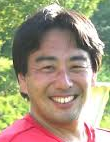
\includegraphics[height=\linewidth/2]{yugo.png}
    \caption{画像テスト}
    \label{fig:YUGO}
  \end{figure}
  \par


\section{先行研究}
  リモートセンシング技術による斜面崩壊・浸水領域検出に関する研究を以下に示す。
  
\subsection{衛星画像を用いた斜面崩壊領域検出}
  江口ら\cite{art01}は地震と豪雨災害後の人工衛星画像を用いて斜面崩壊領域を検出する手法を提案している。この手法では人工衛星画像を土砂領域、植生領域、水領域に分類し、国土地理院提供のDEMデータにより斜面でない領域を除去することによって斜面崩壊領域を検出している。この手法では広範囲の解析が可能であり、衛星画像特有の指標にて容易に土地被覆分類ができるという利点がある。しかし、衛星画像は解像度が低く、条件によっては画像自体が取得できない可能性があり、斜面上の道路等の人工物を誤検出するという問題もある。

\subsection{ヘリコプター空撮画像を用いた斜面崩壊領域検出}
  中山\cite{art02}らは地震災害後のヘリコプター空撮画像を用いて斜面崩壊領域を検出する手法を提案している。この手法ではL*a*b*表色系{}にて土砂領域を検出し、テクスチャ特徴の一つである異質度{}とDEMデータにて道路や平地を除去している。この手法では解像度の高さを利用した異質度にて人工物を除去することができるという利点がある。しかし,位置情報を含む衛星画像と比べ、DEMとの位置合わせの際にずれが生じるという問題がある.

\subsection{ドローン空撮画像を用いた斜面崩壊領域検出}
  機械学習使うやつ
  精度高い
  データ数が少なく、手に入りにくいという問題がある.

\subsection{衛星画像を用いた浸水領域検出}
  なんか津波とかあったかも

\subsection{ヘリコプター空撮画像を用いた浸水領域検出}
  雨宮\cite{art03}らは豪雨災害後のヘリコプター空撮画像を用いて浸水領域を検出する手法を提案している。この手法ではDEMとエッジ抽出{}、テクスチャ特徴の一つである異質度を用いて、エッジ抽出率と異質度が低く凹地となっている領域を浸水領域として検出している。この手法では しかし、建物領域を検出する際

  L*a*b*表色系{}にて土砂領域を検出し、テクスチャ特徴の一つである異質度{}とDEMデータにて道路や平地を除去している。この手法では解像度の高さを利用した異質度にて人工物を除去することができるという利点がある。しかし,位置情報を含む衛星画像と比べ、DEMとの位置合わせの際にずれが生じるという問題がある.


\section{本研究の目的} 
  以上の背景と先行研究を踏まえ、本研究ではDEMと機械学習を用いずに災害後のドローン空撮映像を用いた斜面崩壊・浸水領域を検出する手法を提案する。衛星画像とヘリコプター空撮画像が使用不可能な場合の代替手段として、ドローン空撮画像にて災害領域を同等の精度で検出することを目的とする。


\section{本論文の構成}
  \label{sec:本論文の構成}
  本論文の構成を以下に示す. \par
  第1章では本研究の背景,先行研究,及び目的について述べた.\par
  第2章では本研究の提案手法について述べる.\par
  第3章では実験方法及び実験結果について述べる.\par
  第4章ではまとめとして結論及び今後の課題について述べる.

\end{document}
